\chapter{Elméleti háttér} 
\label{ch:theory}

Ebben a fejezetben a dolgozathoz kapcsolódó fogalmakat és elméleti alapokat mutatom be. Először magának a zenének a releváns tulajdonságairól ejtek szót. Ezután ismertetem a MIR kutatási területet, amelybe dolgozatom is tartozik. Majd végül a mesterséges intelligencián alapuló megoldásokról nyújtok elméleti bevezetőt, érintve a hagyományos gépi tanulás és a mély tanulás módszereit is.

\section{Zene és reprezentációi} 

\subsection{Zene fogalma, tulajdonságai}

A zene egy meglehetősen összetett fogalom. Az ember számára a zene megjelenhet hang formájában, leírhatjuk őket szimbólumok segítségével egy kottában, előfordulhat szöveges formában dalszövegként, képi formában egy albumborító, vagy egy zenész képében, illetve mozdulatokban egy zenei előadás keretében. 

//TODO
Often music means the audio content, although otherwise its scope extends to other types of musical infor-
mation e.g., lyrics, music metadata, or user listening history.

\subsection{Hang reprezentációk}

A hangok fizikai mivoltukban rezgésekként jelennek meg. A rezgéseket matematikailag olyan folytonos függvényekkel tudjuk leírni, melyek értelmezési tartománya az idő, értékkészlete pedig a nyugalmi állapothoz viszonyított pillanatnyi kitérés. Ilyen lehet például egy szinuszgörbe. Ahhoz, hogy a hangokat számítógépen tudjuk tárolni és feldolgozni, ezeket a függvényeket kell ábrázolnunk.  Mivel azonban a számítógép számábrázolása véges, ezért a hangokat először digitalizálni kell. Ez azt jelenti, hogy a folytonos függvényeket diszkrét, azaz véges helyen vett és véges értékekkel rendelkező fügvényekké alakítjuk. Ez úgy történik, hogy ez eredeti függvényünkből megadott időközönként mintát veszünk, diszkrét értékre kerekítjük, és ezeket az értékeket összefűzzük. Az így kapott függvény lesz a hang digitális reprezentációja.
\begin{figure}[H]
  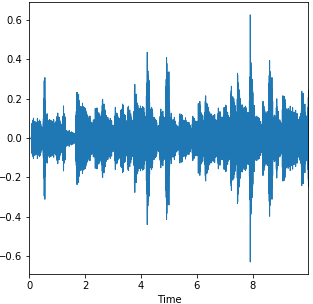
\includegraphics[width=\textwidth]{wave.png}
  \caption{Tíz másodperces hanganyag dipitális reprezentációja}
\end{figure}

A hangok digitális reprezentációja tehát lényegében egydimenziós, mivel egy függvénygörbének tekinthetjük. Ezt szokták hívni nyers hangnak is, ugyanis további reprezentációkká tudjuk transzformálni. A MIR területen megjelenő mély tanulási megoldások jelentős része ezen nyers hangábrázolás helyett inkább a kétdimenziós reprezentációkat alkalmazza bemenetként. Ezt azzal indokolják, hogy a nyers bemeneten való tanítás sikeréhez nagyobb adathalmaz szükséges, mint a kétdimenziós reprezentációkéhoz. \cite{Choi2017}

//TODO 2d reprezentációk


\subsection{Music Information Retrieval (MIR)} 

A bevezetőben már említettem a zenei információk kinyerését (music information retrieval - MIR). Ez egy interdiszciplináris kutatási terület, magában hordozza többek között a zeneelmélet, pszichoakusztika, pszichológia, informatika, jelfeldolgozás és gépi tanulás tudományágakat. Céljára jól utal az elnevezése, zenékből szeretnénk releváns információt kinyerni, és ezeket felhasználni \cite{Choi2017}. A felhasználásra szerintem nagyon jó, életszerű példát ad Downie 2003-as cikkének \cite{Downie2003} bevezetője, amelyet a következőképp fordíthatunk le:

''Képzeljünk el egy világot, ahol egyszerűen felénekelhetjük egy számítógépnek a dalrészletet, ami már reggeli óta a fejünkben jár. A gép elfogadja a hamis énekünket, kijavítja, és azonnal javaslatot tesz arra, hogy éppen a ''Camptown Races'' című számra gondoltunk. Miután mi belehallgatunk a gép által talált számos relevánsnak tartott MP3 fájl egyikébe, elfogadhatjuk a gép javaslatát. Ezután elégedetten elutasíthatjuk a felajánlást, hogy az összes további létező verzióját is felkutassa a dalnak, ide értve a nemrég megjelent olasz rap verziót, vagy a skótdudás duettre írt kottát.''  \cite{Downie2003}

Figyeljük meg, hogy ez a hétköznapi eset mennyire össztett probléma. A következő feladatok jelennek meg:
\begin{itemize}
\item Az emberi éneklés, vagy dúdolás alapján hangfelismerés.
\item Hang alapú lekérdezés egy zenei adatbázisban az előbbi bemenettel.
\item Hangelemzés, feldolgozás, hogy a hamis hangokat ki tudjuk javítani, az esetleges háttérzajokat eltávolítsuk, illetve ha kell, a dallamból automatikusan kottát generáljunk.
\item Hasonlóságon alapuló keresés zenék között, hogy megtaláljuk a kívánt dalt az adatbázisban.
\item Zenei feldolgozások detektálása, hogy további verzióit is megtaláljuk egy adott dalnak.
\end{itemize}

MIR problémák definiálását több szempontból közelíthetjük meg. Choi cikke \cite{Choi2017} két tengelyre osztja fel a problémateret: szubjektivitás és eldöntési időmérték. A szubjektivitás tengelyen léteznek szubjektívebb feladatok, melyekre nincsenek egyértelmű válaszok. Ilyen lehet például a zene műfajának meghatározása. Objektívebb feladatoknak tekinthetjük azokat, melyek eredménye egyértelműen meghatárhozható, esetleg számszerűsíthető. Ide tartozik a hangszerfelismerés, vagy a tempó észlelés. \cite{Choi2017}

A másik tengely, az eldöntési időmérték aszerint sorolja be a feladatokat, hogy mekkora időegységeken értelmezhető egy becslés. Ez egy relatív mérték. Például a dallamfelismerés eldöntési időmértékére azt mondhatjuk, hogy alacsony, mert egy felismert dallam jó eséllyel nem fedi le az egész zenét. Másik kifejezéssel azt mondhatjuk, hogy ez egy időben változó, azaz dinamikus tulajdonság. Ellenben a tempó általában állandó értékű az egész zenében, így a teljes zeneszámot fel tudjuk címkézni egy adott tempóval. Erre azt mondjuk, hogy eldöntési időmértéke relatív magas, azaz ez egy statikus tulajdonsága a zenének.\cite{Choi2017}

A hangszerfelismerést tekinthetjük statikus, illetve dinamikus feladatnak is a probléma megközelítésének függvényében. Dinamikus, ha erős címkézést szeretnénk megvalósítani, tehát arra vagyunk kíváncsiak, hogy adott időpillanatban éppen milyen hangszerek szólalnak meg. Gyenge címkézés esetén viszont a feladat statikussá válik. Ebben az esetben az egész zenére vetítve szeretnénk címkéket kapni egyes hangszerek jelenlétével, vagy a többi hangszerrel szembeni dominanciájával kapcsolatban.

TODO több MIR feladat


\section{Mesterséges intelligencia}

A mesterséges intelligencia egy általános fogalom az emberi gondolkodás számítógéppel való reprodukálására történő módszerekre. Ahogy arról a bevezetésben is szót ejtettem, a MIR tudományág gyakran használ mesterséges intelligencián alapuló megoldásokat. A továbbiakban két mesterséges intelligenciát megvalósító módszert mutatok be röviden: elsőként a gépi tanulást, majd a mély tanulást, amely a gépi tanulás egy ágazata és napjaink meghatározó trendje. \cite{ai}

\begin{figure}[H]
  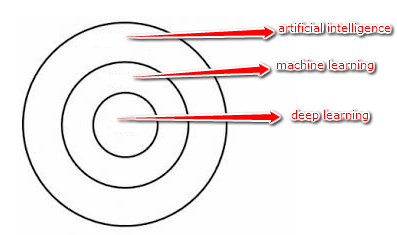
\includegraphics{ai.png}
  \caption{Egyes fogalmak közti tartalmazás szemléltetve, forrás: \cite{ai} }
\end{figure}

\subsection{Gépi tanulás (machine learning)}

A gépi tanulás tehát a mesterséges intelligencia megvalósításának egy módszere. Lényege, hogy explicit utasításokat tartalmazó program helyett a bemeneti adatokat egy tanító algoritmusnak adjuk át. Ha elég mennyiségű és minőségű adatot szolgáltatunk a tanításhoz, akkor a modellünk 

Hagyományos gépi tanulásról beszélünk, amikor 

//TODO


\subsection{Mély tanulás (deep learning)}

A mély tanulás gyakorlatilag a gépi tanulás egy részhalmaza. 

//TODO  miben más mint az ML, architektúrák stb